
\documentclass[10pt,a4paper]{article}
\usepackage[T1]{fontenc}
\usepackage{tikz}
\usepackage[margin=1cm]{geometry}
\begin{document}
\section*{Binary Tree Construction Steps}
This document illustrates the step-by-step construction of a binary tree. Each step shows the tree after the insertion of a new node, demonstrating how the tree evolves over time.

\subsection*{Algorithm Description}
The binary tree is constructed using a level-order insertion method. This means that new nodes are added starting from the top level, filling in from left to right. If a node has a left and right child, the insertion continues to the next level. The process repeats until all nodes are inserted into the tree.

\subsection*{Step-by-Step Visualization}
The following figures represent the state of the binary tree after each insertion step. The captions describe the order of the steps. Nodes are represented by circles, and the connections between them indicate the parent-child relationships.

\begin{figure}[h!]
\centering

\begin{minipage}{0.8\textwidth}
    \centering
    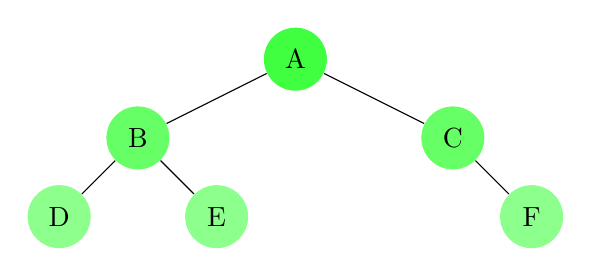
\begin{tikzpicture}[level distance=10mm]
        \tikzstyle{every node}=[fill=green!75,circle,inner sep=1pt, minimum size=8mm]
        \tikzstyle{level 1}=[sibling distance=40mm, set style={{every node}+=[fill=green!60]}]
        \tikzstyle{level 2}=[sibling distance=20mm, set style={{every node}+=[fill=green!45]}]
        \tikzstyle{level 3}=[sibling distance=15mm, set style={{every node}+=[fill=green!30]}]
        \tikzstyle{level 4}=[sibling distance=10mm, set style={{every node}+=[fill=green!15]}]
        \node {A} child {node {B} child {node {D} } child {node {E} }} child {node {C} child[fill=none] {edge from parent[draw=none]} child {node {F} }};
    \end{tikzpicture}
    \caption{Initial Tree}
\end{minipage}
\vspace{1cm}

\begin{minipage}{0.8\textwidth}
    \centering
    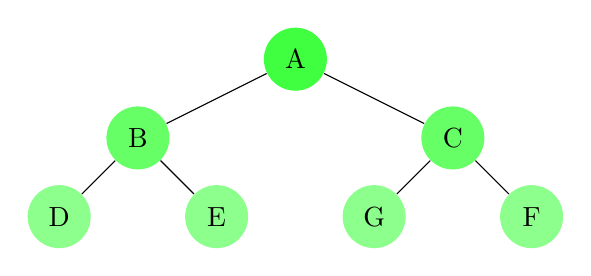
\begin{tikzpicture}[level distance=10mm]
        \tikzstyle{every node}=[fill=green!75,circle,inner sep=1pt, minimum size=8mm]
        \tikzstyle{level 1}=[sibling distance=40mm, set style={{every node}+=[fill=green!60]}]
        \tikzstyle{level 2}=[sibling distance=20mm, set style={{every node}+=[fill=green!45]}]
        \tikzstyle{level 3}=[sibling distance=15mm, set style={{every node}+=[fill=green!30]}]
        \tikzstyle{level 4}=[sibling distance=10mm, set style={{every node}+=[fill=green!15]}]
        \node {A} child {node {B} child {node {D} } child {node {E} }} child {node {C} child {node {G} } child {node {F} }};
    \end{tikzpicture}
    \caption{Step 2}
\end{minipage}
\vspace{1cm}

\begin{minipage}{0.8\textwidth}
    \centering
    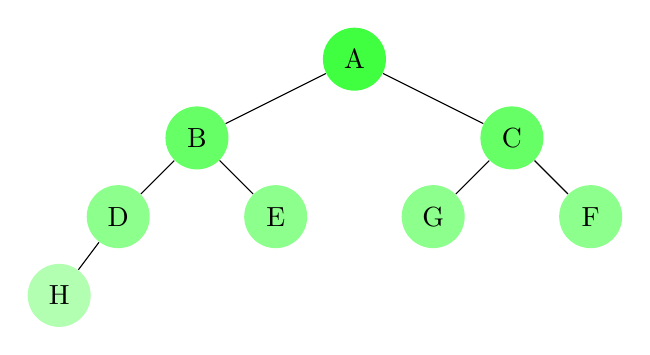
\begin{tikzpicture}[level distance=10mm]
        \tikzstyle{every node}=[fill=green!75,circle,inner sep=1pt, minimum size=8mm]
        \tikzstyle{level 1}=[sibling distance=40mm, set style={{every node}+=[fill=green!60]}]
        \tikzstyle{level 2}=[sibling distance=20mm, set style={{every node}+=[fill=green!45]}]
        \tikzstyle{level 3}=[sibling distance=15mm, set style={{every node}+=[fill=green!30]}]
        \tikzstyle{level 4}=[sibling distance=10mm, set style={{every node}+=[fill=green!15]}]
        \node {A} child {node {B} child {node {D} child {node {H} } child[fill=none] {edge from parent[draw=none]}} child {node {E} }} child {node {C} child {node {G} } child {node {F} }};
    \end{tikzpicture}
    \caption{Step 3}
\end{minipage}
\vspace{1cm}

\begin{minipage}{0.8\textwidth}
    \centering
    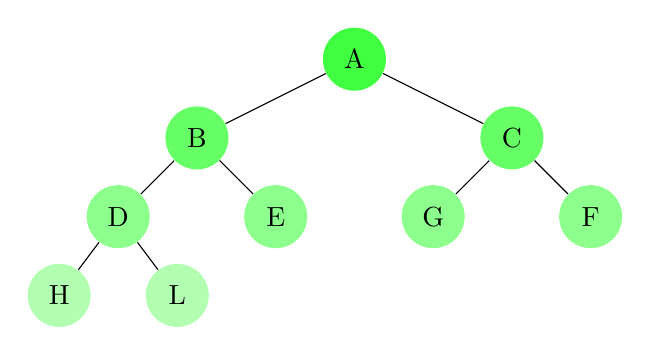
\begin{tikzpicture}[level distance=10mm]
        \tikzstyle{every node}=[fill=green!75,circle,inner sep=1pt, minimum size=8mm]
        \tikzstyle{level 1}=[sibling distance=40mm, set style={{every node}+=[fill=green!60]}]
        \tikzstyle{level 2}=[sibling distance=20mm, set style={{every node}+=[fill=green!45]}]
        \tikzstyle{level 3}=[sibling distance=15mm, set style={{every node}+=[fill=green!30]}]
        \tikzstyle{level 4}=[sibling distance=10mm, set style={{every node}+=[fill=green!15]}]
        \node {A} child {node {B} child {node {D} child {node {H} } child {node {L} }} child {node {E} }} child {node {C} child {node {G} } child {node {F} }};
    \end{tikzpicture}
    \caption{Step 4}
\end{minipage}
\vspace{1cm}

\end{figure}
\newpage

\begin{figure}[h!]
\centering

\begin{minipage}{0.8\textwidth}
    \centering
    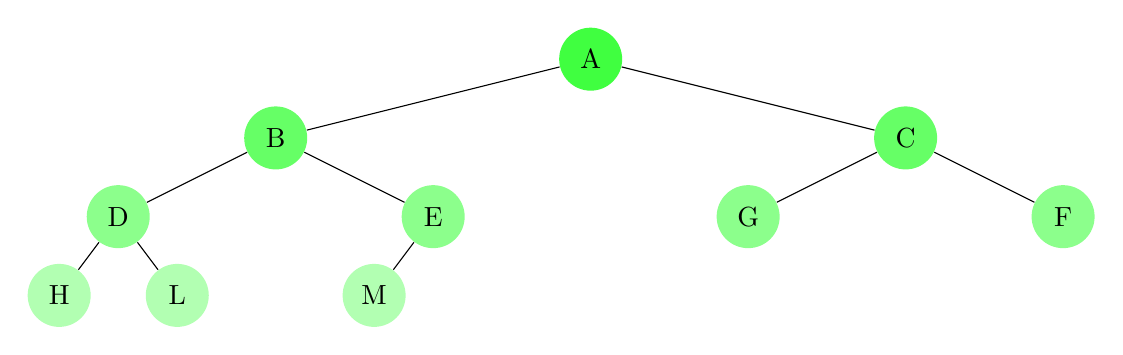
\begin{tikzpicture}[level distance=10mm]
        \tikzstyle{every node}=[fill=green!75,circle,inner sep=1pt, minimum size=8mm]
        \tikzstyle{level 1}=[sibling distance=80mm, set style={{every node}+=[fill=green!60]}]
        \tikzstyle{level 2}=[sibling distance=40mm, set style={{every node}+=[fill=green!45]}]
        \tikzstyle{level 3}=[sibling distance=15mm, set style={{every node}+=[fill=green!30]}]
        \tikzstyle{level 4}=[sibling distance=10mm, set style={{every node}+=[fill=green!15]}]
        \node {A} child {node {B} child {node {D} child {node {H} } child {node {L} }} child {node {E} child {node {M} } child[fill=none] {edge from parent[draw=none]}}} child {node {C} child {node {G} } child {node {F} }};
    \end{tikzpicture}
    \caption{Step 5}
\end{minipage}
\vspace{1cm}

\begin{minipage}{0.8\textwidth}
    \centering
    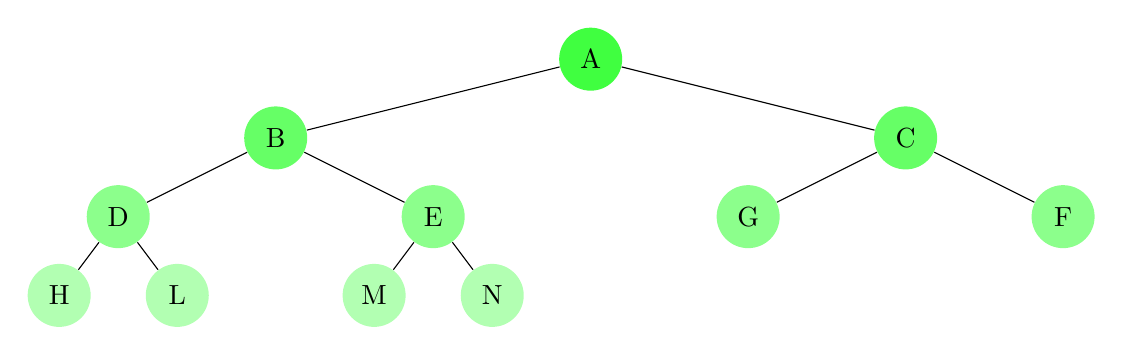
\begin{tikzpicture}[level distance=10mm]
        \tikzstyle{every node}=[fill=green!75,circle,inner sep=1pt, minimum size=8mm]
        \tikzstyle{level 1}=[sibling distance=80mm, set style={{every node}+=[fill=green!60]}]
        \tikzstyle{level 2}=[sibling distance=40mm, set style={{every node}+=[fill=green!45]}]
        \tikzstyle{level 3}=[sibling distance=15mm, set style={{every node}+=[fill=green!30]}]
        \tikzstyle{level 4}=[sibling distance=10mm, set style={{every node}+=[fill=green!15]}]
        \node {A} child {node {B} child {node {D} child {node {H} } child {node {L} }} child {node {E} child {node {M} } child {node {N} }}} child {node {C} child {node {G} } child {node {F} }};
    \end{tikzpicture}
    \caption{Step 6}
\end{minipage}
\vspace{1cm}

\begin{minipage}{0.8\textwidth}
    \centering
    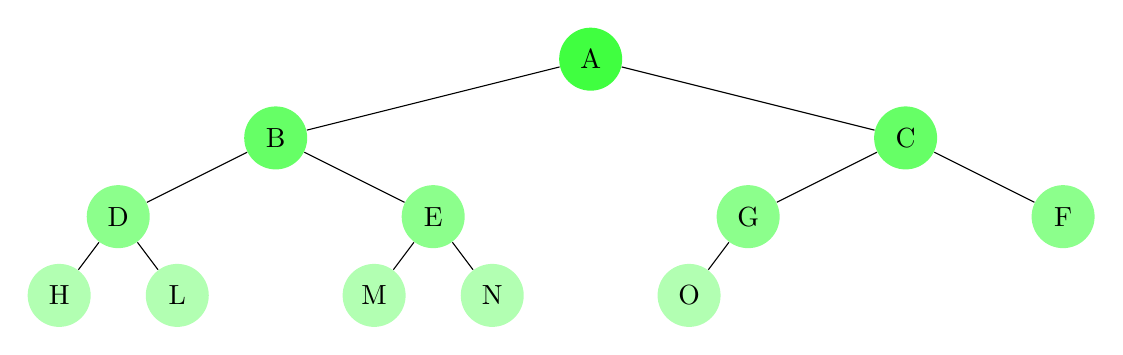
\begin{tikzpicture}[level distance=10mm]
        \tikzstyle{every node}=[fill=green!75,circle,inner sep=1pt, minimum size=8mm]
        \tikzstyle{level 1}=[sibling distance=80mm, set style={{every node}+=[fill=green!60]}]
        \tikzstyle{level 2}=[sibling distance=40mm, set style={{every node}+=[fill=green!45]}]
        \tikzstyle{level 3}=[sibling distance=15mm, set style={{every node}+=[fill=green!30]}]
        \tikzstyle{level 4}=[sibling distance=10mm, set style={{every node}+=[fill=green!15]}]
        \node {A} child {node {B} child {node {D} child {node {H} } child {node {L} }} child {node {E} child {node {M} } child {node {N} }}} child {node {C} child {node {G} child {node {O} } child[fill=none] {edge from parent[draw=none]}} child {node {F} }};
    \end{tikzpicture}
    \caption{Step 7}
\end{minipage}
\vspace{1cm}

\end{figure}
\newpage

\end{document}
